% begin module parametric-ex2
\begin{frame}
\begin{example} %[Example 2, p. 658]
Sketch and identify the curve defined by the parametric equations
\abovedisplayskip=2pt
\belowdisplayskip=2pt
\[
\alert<handout:0| 15>{x = \cos t}, \qquad \alert<handout:0| 14>{y = \sin t}.
\]
\begin{columns}[c]
\column{.55\textwidth}

\psset{xunit=2, yunit=2cm}
\begin{pspicture}(-1.5, -1.5)(1.5,1.5)

\tiny
\fcAxesStandard{-1.4}{-1.4}{1.4}{1.4}

\fcXTick{1}
\rput[rb](0.95, 0.05){$(1,0)$}

%Calculator input for full circle: plotCurve{}(\cos{}t, \sin{}t, 0, 2 \pi)
\uncover<handout:0| 3->{
\fcFullDot{1}{0}
\rput[bl](1.05, 0.05){$t=0$}
}

\uncover<handout:0| 5->{
\parametricplot[arrows=->, linecolor=\fcColorGraph, plotpoints=200] {0} {0.261799388}{t 57.29578 mul cos t 57.29578 mul sin }
\parametricplot[ linecolor=\fcColorGraph, plotpoints=200] {0.261799388} {0.523598776}{t 57.29578 mul cos t 57.29578 mul sin }
\rput[bl](0.9, 0.5){$t=\frac{\pi}{6}$}
\fcFullDot{0.866025} {0.500000}
}

\uncover<handout:0| 7->{
\tiny
%Calculator input: plotCurve{}(\cos{}t, \sin{}t, 1/4 \pi, 1/3 \pi)
\parametricplot[linecolor=\fcColorGraph, plotpoints=1000]{0.785398}{1.0472}{t 57.29578 mul cos t 57.29578 mul sin }
%Calculator input: plotCurve{}(\cos{}t, \sin{}t, 1/6 \pi, 1/4 \pi)
\parametricplot[arrows=->, linecolor=\fcColorGraph, plotpoints=1000]{0.523599}{0.785398}{t 57.29578 mul cos t 57.29578 mul sin }
\fcFullDot{0.500000}{0.866025}
\rput[bl](0.55, 0.9){$t=\frac{\pi}{3}$}
}
\uncover<handout:0| 9->{
%Calculator input: plotCurve{}(\cos{}t, \sin{}t, 5/12 \pi, 1/2 \pi)
\parametricplot[linecolor=\fcColorGraph, plotpoints=1000]{1.309}{1.5708}{t 57.29578 mul cos t 57.29578 mul sin }
%Calculator input: plotCurve{}(\cos{}t, \sin{}t, 1/3 \pi, 5/12 \pi)
\parametricplot[arrows=->, linecolor=\fcColorGraph, plotpoints=1000]{1.0472}{1.309}{t 57.29578 mul cos t 57.29578 mul sin }
\fcFullDot{0.000000}{ 1.000000}
\rput[bl](0.1, 1.05){$t=\frac{\pi}{2}$}
}
\uncover<handout:0| 11->{
%Calculator input: plotCurve{}(\cos{}t, \sin{}t, 3/4 \pi, \pi)
\parametricplot[linecolor=\fcColorGraph, plotpoints=1000]{2.35619}{3.14159}{t 57.29578 mul cos t 57.29578 mul sin }
%Calculator input: plotCurve{}(\cos{}t, \sin{}t, 1/2 \pi, 3/4 \pi)
\parametricplot[arrows=->, linecolor=\fcColorGraph, plotpoints=1000]{1.5708}{2.35619}{t 57.29578 mul cos t 57.29578 mul sin }
\fcFullDot{-1}{0}
\rput[rb](-1, 0.1){$t=\pi$}
}
\uncover<handout:0| 13->{
%Calculator input: plotCurve{}(\cos{}t, \sin{}t, 5/4 \pi, 3/2 \pi)
\parametricplot[linecolor=\fcColorGraph, plotpoints=1000]{3.92699}{4.71239}{t 57.29578 mul cos t 57.29578 mul sin }
%Calculator input: plotCurve{}(\cos{}t, \sin{}t, \pi, 5/4 \pi)
\parametricplot[arrows=->, linecolor=\fcColorGraph, plotpoints=1000]{ 3.14159} {3.92699}{t 57.29578 mul cos t 57.29578 mul sin }
\fcFullDot{0}{-1}
\rput[tr](-0.1, -1.05){$t=\frac{3\pi}{2}$}
}
\uncover<handout:0| 15->{
%Calculator input: plotCurve{}(\cos{}t, \sin{}t, 7/4 \pi, 2 \pi)
\parametricplot[linecolor=\fcColorGraph, plotpoints=1000 ]{ 5.49779}{6.28319}{t 57.29578 mul cos t 57.29578 mul sin }
%Calculator input: plotCurve{}(\cos{}t, \sin{}t, 3/2 \pi, 7/4 \pi)
\parametricplot[arrows=->, linecolor=\fcColorGraph, plotpoints=1000]{4.71239}{5.49779}{t 57.29578 mul cos t 57.29578 mul sin }
\rput[tl](1, -0.1){$t=2\pi$}
}
\end{pspicture}

%\ \only<handout:0| -2>{%
%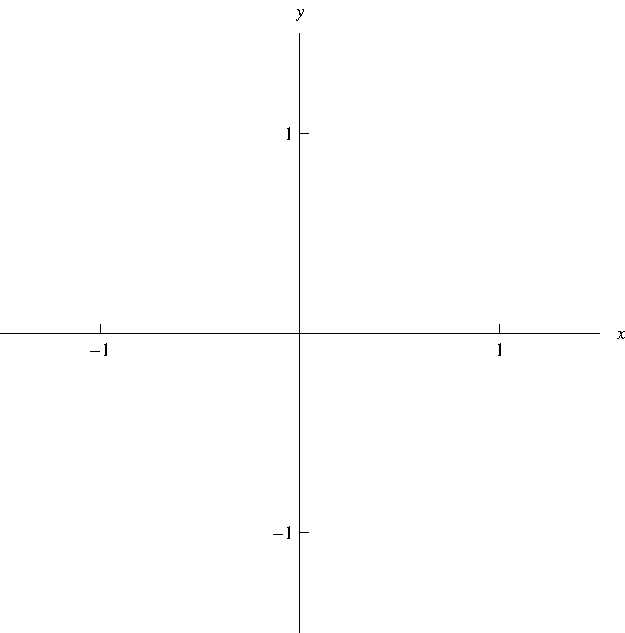
\includegraphics[height=6cm]{parametric-curves/pictures/11-01-ex2a.pdf}%
%}%
%\only<handout:0| 3-4>{%
%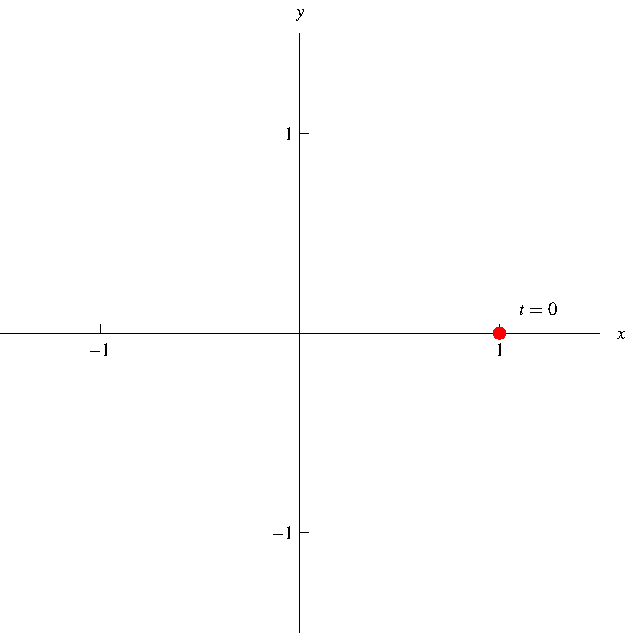
\includegraphics[height=6cm]{parametric-curves/pictures/11-01-ex2b.pdf}%
%}%
%\only<handout:0| 5-6>{%
%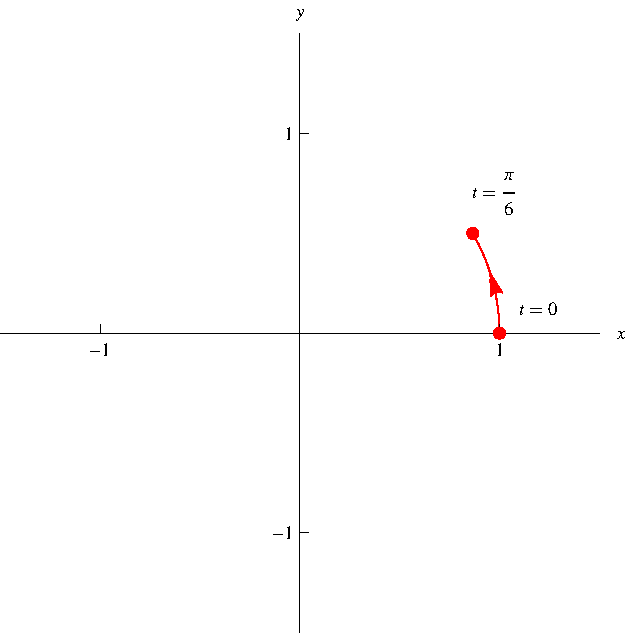
\includegraphics[height=6cm]{parametric-curves/pictures/11-01-ex2c.pdf}%
%}%
%\only<handout:0| 7-8>{%
%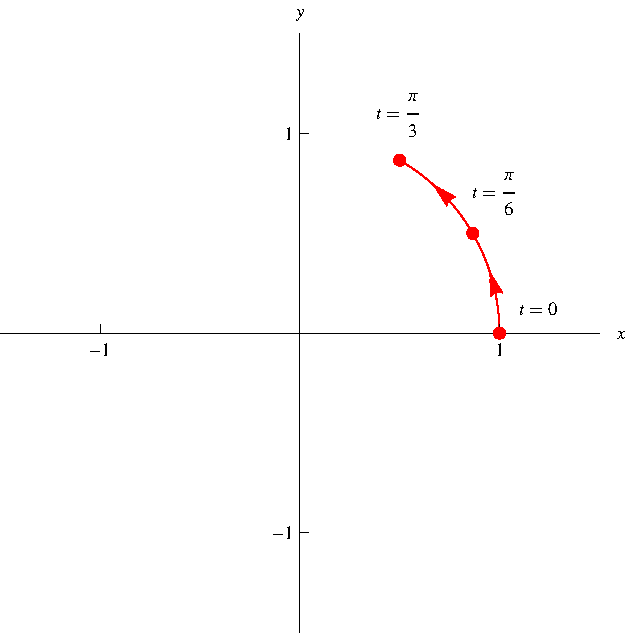
\includegraphics[height=6cm]{parametric-curves/pictures/11-01-ex2d.pdf}%
%}%
%\only<handout:0| 9-10>{%
%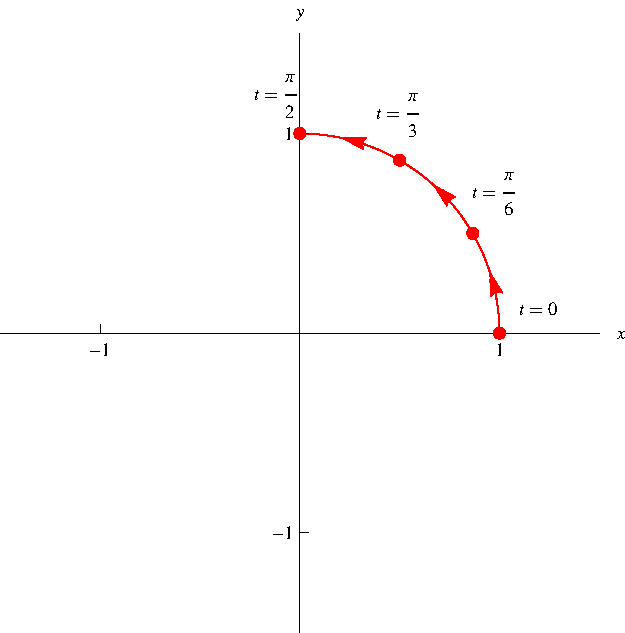
\includegraphics[height=6cm]{parametric-curves/pictures/11-01-ex2e.pdf}%
%}%
%\only<handout:0| 11-12>{%
%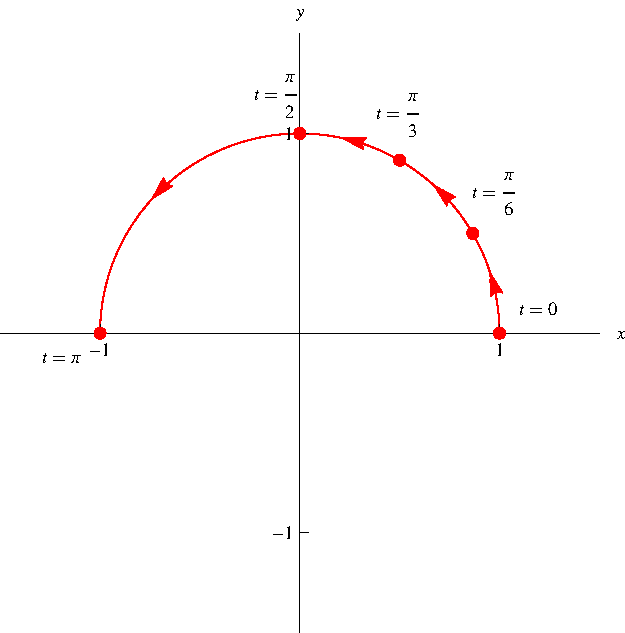
\includegraphics[height=6cm]{parametric-curves/pictures/11-01-ex2f.pdf}%
%}%
%\only<handout:0| 13-14>{%
%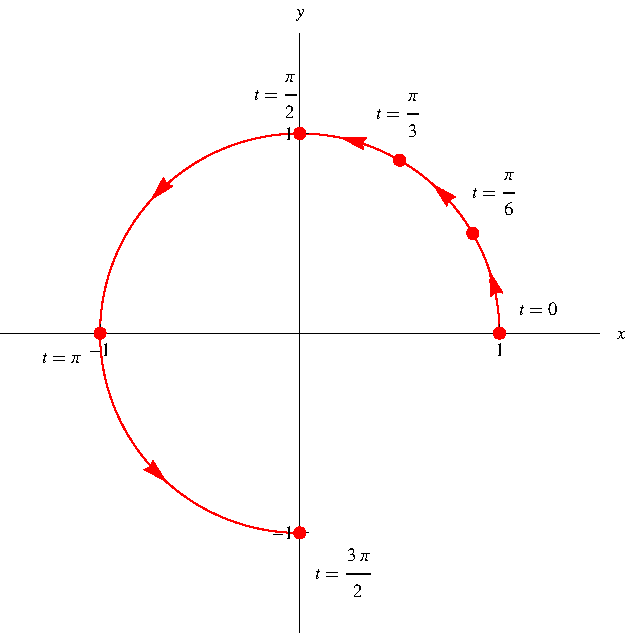
\includegraphics[height=6cm]{parametric-curves/pictures/11-01-ex2g.pdf}%
%}%
%\only<15->{%
%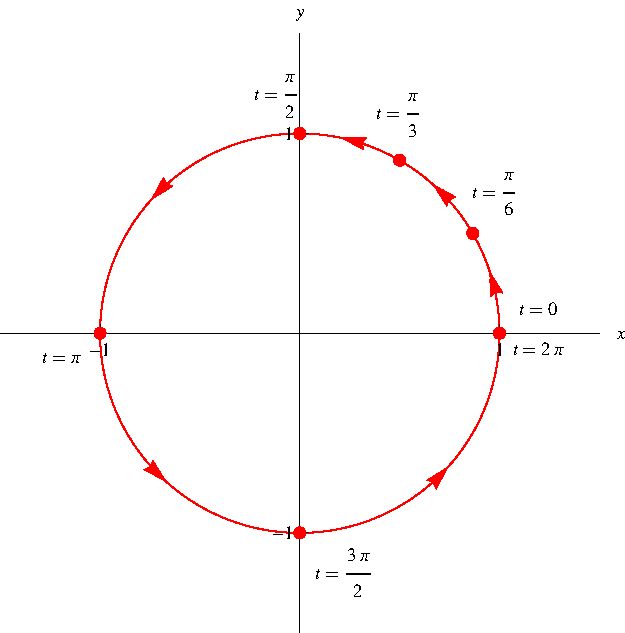
\includegraphics[height=6cm]{parametric-curves/pictures/11-01-ex2h.pdf}%
%}%

\column{.45\textwidth}
\[
\begin{array}{|r|r|r|}
\hline
t & x & y\\
\hline
\alert<handout:0| 2-3>{0} &%
\alert<handout:0| 2-3>{\uncover<3->{1}} &%
\alert<handout:0| 2-3>{\uncover<3->{0}} \\%
\alert<handout:0| 4-5>{\frac{\pi}6} &%
\alert<handout:0| 4-5>{\uncover<5->{\frac{\sqrt{3}}{2}}} &%
\alert<handout:0| 4-5>{\uncover<5->{\frac12}} \\%
\alert<handout:0| 6-7>{\frac{\pi}3} &%
\alert<handout:0| 6-7>{\uncover<7->{\frac12}} &%
\alert<handout:0| 6-7>{\uncover<7->{\frac{\sqrt{3}}2}} \\%
\alert<handout:0| 8-9>{\frac{\pi}2} &%
\alert<handout:0| 8-9>{\uncover<9->{0}} &%
\alert<handout:0| 8-9>{\uncover<9->{1}} \\%
\alert<handout:0| 10-11>{\pi} &%
\alert<handout:0| 10-11>{\uncover<11->{-1}} &%
\alert<handout:0| 10-11>{\uncover<11->{0}} \\%
\alert<handout:0| 12-13>{\frac{3\pi}2} &%
\alert<handout:0| 12-13>{\uncover<13->{0}} &%
\alert<handout:0| 12-13>{\uncover<13->{-1}} \\%
\alert<handout:0| 14-15>{2\pi} &%
\alert<handout:0| 14-15>{\uncover<15->{1}} &%
\alert<handout:0| 14-15>{\uncover<15->{0}} \\%
\hline
\end{array}
\]
\abovedisplayskip=2pt
\belowdisplayskip=2pt
\[
\uncover<16->{%
x^2 + y^2 = %
}%
\uncover<17->{%
\cos^2 t+ \sin^2 t = %
}%
\uncover<18->{%
1%
}%
\]
\uncover<19->{%
Therefore $(x,y)$ travels on the unit circle $x^2 + y^2 = 1$.
}%
\end{columns}
\end{example}
\end{frame}
% end module parametric-ex2
